% Optional Introduction
\chapter{Introduction}
\label{chapter:introduction}

Computer security is an inherently adversarial discipline in which
each ``side'' seeks to exploit the assumptions and limitations of the
other.  Attackers rely on exploiting knowledge of vulnerabilities,
configuration errors or operational lapses in order to penetrate
targeted systems, while defenders in turn seek to improve their
resistance to such attacks by better understanding the nature of
contemporary threats and the technical fingerprints left by attacker's
craft.  Invariably, this means that attackers are driven to innovate
and diversify while defenders, in response, must continually monitor
for such changes and update their operational security practices
accordingly.  This dynamic is present in virtually every aspect of the
operational security landscape, from anti-virus signatures to the
configuration of firewalls and intrusion detection systems to incident
response and triage.  Common to all such reifications, however, is the
process of monitoring for new data on attacker behavior and using that
data to update defenses and security practices. Indeed, the extent to
which a defender is able to gather and analyze such data effectively
defines a de facto window of vulnerability---the time during which an
organization is less effective in addressing attacks due to ignorance
of current attacker behaviors.

This abstract problem has given rise to a concrete demand for
contemporary threat data sources that are frequently collectively
referred to as \emph{threat intelligence}. Threat intelligence 
is the \emph{knowledge} that allows organizations to understand and 
mitigate cyber-attacks. This ``knowledge'' involves a wide variety 
of things. It can be vulnerability reports, where system and 
network administrators can learn the vulnerabilities and the potential
impact on their systems. It can also be IP or domain blacklists,
which report the sources where attacks originate from, so people
can take precautions against these indicators. It can even be an 
online discussion thread in an underground forum, so security 
experts can track what malicious actors are discussing. 
All of this knowledge captures contemporary information about potential 
threats, and therefore helps organizations better defend 
against them.

By far the most common form of threat intelligence are so-called 
\emph{indicators of compromise:} simple observable behaviors that 
signal that a host or network may be compromised. These indicators 
are in general straightforward forensic data that are directly 
associated with attacks. The most notable examples are:
\begin{prettylist}
    \item \textbf{IP Addresses}: IPs known to launch certain 
    attacks, like port scanning, vulnerability probing, brute-force login, etc.
    \item \textbf{Domains}: Domains known to host 
    malware Command-and-Control servers or sending spam emails, etc.
    \item \textbf{URLs}: Compromised websites or phish URLs, etc.
    \item \textbf{File Hashes}: Indicating a file or executable 
    known to be associated with a particular variety of malware, etc.
\end{prettylist}

The presence of such indicators in a system or network is a symptom 
that alerts an organization to a problem. For example, if one 
machine in an organization communicated with a domain known to be
associated with malware Command-and-Control servers, it is a strong
indication that this machine is probably infected with the 
corresponding malware. Part of an organization's defenses 
should reasonably include monitoring its assets
for such indicators to detect and mitigate potential compromises as
they occur. And these indicators are simple enough that they can be
easily integrated into defense or monitoring systems, like network
firewalls or malware scanners.

While each organization naturally collects a certain amount of threat
intelligence data on its own (e.g., the attacks they repel, the e-mail
spam they filter, etc.), any single entity has a limited footprint and
few are instrumented to carefully segregate crisp signals of attacks
from the range of ambiguity found in normal production network and
system logs. Thus, it is now commonly accepted that threat
intelligence data procurement is a specialized activity whereby
third-party firms, and/or collections of public groups, employ a range
of monitoring techniques to aggregate, filter and curate quality
information about current threats.  Indeed, the promised operational
value of threat intelligence has created a thriving (multi-billion
dollar) market~\cite{timarket}. 

Most established security firms, such as Cisco Security~\cite{ciscotalos}, 
Palo Alto Networks~\cite{panautofocus}, Fortinet~\cite{fortinet}, 
and many specialized companies, including CrowdStrike~\cite{crowdstrike}, 
Anomali ThreatStream~\cite{anomali}, Recorded Future~\cite{recordedfuture}, 
are all offering threat intelligence solutions. Public threat
intelligence providers like Spamhaus, Abuse.ch, Dshield etc, are also 
getting more and more attention. The global threat intelligence market is
predicated to surpass \$13 Billion in 2025~\cite{tipredict2018}. With the
industry thriving, there is also a rapid increase in the related research
works~\cite{tounsi2018survey}, covering topics from data characterizing,
effectiveness evaluation to designing better sharing systems and protocols.

From a high level, there are two major aspects of threat intelligence: 
\textit{Data} and \textit{Usage}. \textit{Data} represents the content 
of threat intelligence---the actual information provided in different threat
intelligence products. \textit{Usage}, on the other hand, represents 
different ways people can use threat intelligence to help. Therefore, 
all research surrounding threat intelligence can be categorized into 
these two areas: research related to threat intelligence data itself, 
and studies on different ways to use the data. They are the two sides 
of the same coin.

When looking at these two general aspects, one can further 
take two different research approaches: \textit{Empirical Study} and 
\textit{Algorithm Exploration}. Empirical study focuses on 
understanding the current threat intelligence: analyzing patterns 
in existing data, measuring different use cases, discover shortcomings 
in current data format design, etc. This approach emphasizes measuring 
existing solutions, uncovering patterns and limitations, so the 
community can gain valuable insights. Algorithm exploration, 
on the other hand, focuses on designing new algorithms and new tools to 
improve current solutions, such as new threat hunting algorithms to improve 
threat intelligence data quality, or better ways to utilize these data 
during operation, etc. This approach emphasizes designing new tools,
techniques and approaches to help the community better generate, share, 
and use threat intelligence data.

\begin{figure}
\centering
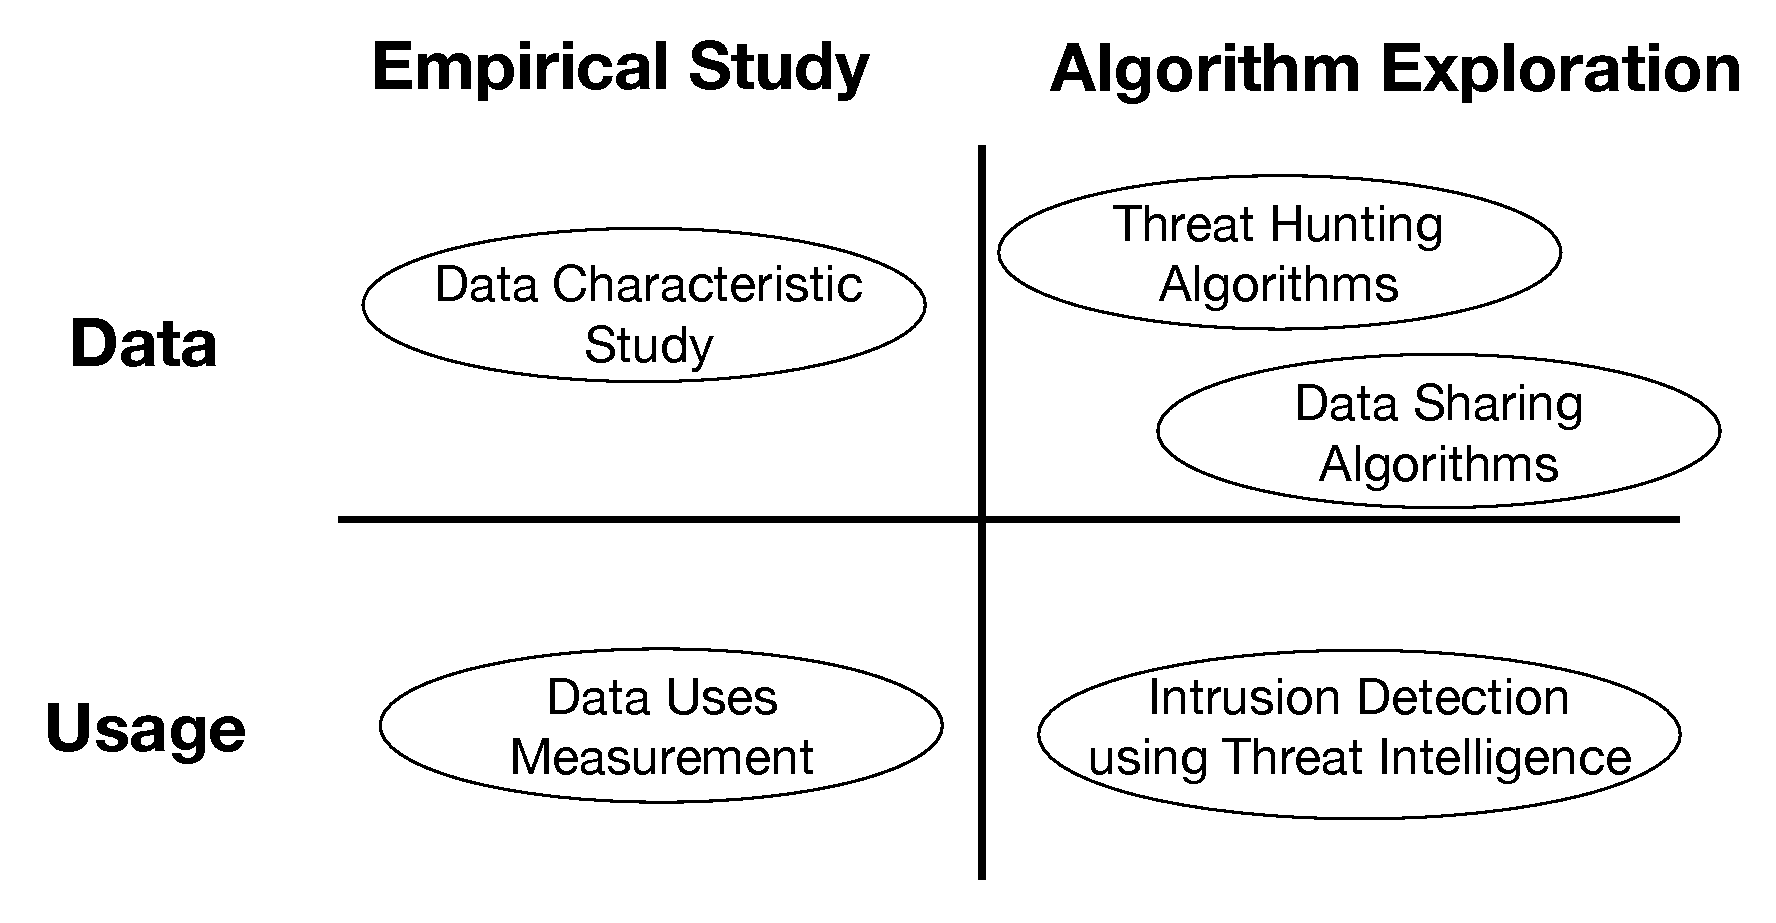
\includegraphics[width=0.8\textwidth]{threat_intel_overview_v2.pdf}
\caption{Threat Intelligence research overview and example research
topics in each direction.}
\label{fig:threat_intel_overview}
\end{figure}

Therefore, threat intelligence research can be divided into four 
different directions (as illustrated in Figure
~\ref{fig:threat_intel_overview}). These are:
\begin{prettylist}
    \item Empirical analysis of threat intelligence data: \\
    Characterizing and understanding threat intelligence data, profiling the 
    systems and techniques used to generate such data, measuring different 
    threat sharing strategies and their effectiveness, etc.
    
    \item Algorithm exploration related to threat intelligence data: \\
    Designing algorithms for threat hunting (threat intelligence generation),
    defining specification for data description and protocols for data 
    sharing, etc.
    
    \item Empirical analysis of threat intelligence usage: \\
    Measuring how organizations use threat intelligence, and understanding
    the impact such uses on the Internet, etc.
    
    \item Algorithm exploration related to threat intelligence usage: \\
    Designing better methods to use threat intelligence during system and 
    network defense (e.g. increasing coverage, reducing false positives),
    exploring new ways to use threat intelligence data, such as for machine
    learning training data, etc.
\end{prettylist}

There have been many previous research works covering various topics in these
four directions. Most of the works focus on threat intelligence generation
techniques (all threat detection techniques, such as malware detection, phish 
detection, causality analysis, etc.) and threat sharing methods (data formats, 
sharing protocols and sharing platforms, etc.). However, few works have taken
the empirical approach and systematically evaluate the existing threat
intelligence, both in terms of the data itself and its usage. Our community 
lacks a concrete understanding of threat intelligence in the real-world.

In this dissertation, I take the empirical approach and explore both the 
\textit{Data} and \textit{Usage} aspects of the threat intelligence
domain. In exploring threat intelligence data (described in
Chapter~\ref{chapter:data_character}), I conduct a comparative analysis on
existing threat intelligence products. In particular, I design formal 
metrics for evaluating threat intelligence data and I used these tools to 
evaluate {\numipfeeds} distinct IP address IoC feeds and {\numhashfeeds}
distinct malware IoC feeds. Through this chapter, I reveal the limitation of
existing threat intelligence data and discuss potential improvements 
based on my findings. In exploring threat intelligence operations 
(described in Chapter~\ref{chapter:data_usage}),
I measure how threat intelligence data is being used on a large scale. 
I design a method using IP ID side channel to infer the connectivity 
between two Internet hosts from a third point. Using this 
method, I conduct a large scale Internet measurement over {\reflroughnum} 
U.S. hosts and establish their use of {\blacklistnum} popular public IP
blacklists. I further investigate a broader use of blacklists among the 
hosts, and discovered over 73K hosts have shown blacklist related blocking 
behavior. Together, my work provides an in-depth look into the current
status of threat intelligence and augments the knowledge of our community
on this topic.

%\verb!\mainmatter! macro because it should start on page~1.
%\end{dissertationintroduction}
